% Created 2020-04-23 Thu 13:35
% Intended LaTeX compiler: pdflatex
\documentclass[presentation,aspectratio=169,smaller]{beamer}
\usepackage[utf8x]{inputenc}
\usepackage[T1]{fontenc}
\usepackage{graphicx}
\usepackage{grffile}
\usepackage{longtable}
\usepackage{wrapfig}
\usepackage{rotating}
\usepackage[normalem]{ulem}
\usepackage{amsmath}
\usepackage{textcomp}
\usepackage{amssymb}
\usepackage{capt-of}
\usepackage{hyperref}
\usepackage{color}
\usepackage[newfloat]{minted}
\usepackage[utf8]{inputenc}
\usepackage{soul}
\usepackage{unicode-math}
\usepackage{mathtools}
\usepackage[mathletters]{ucs}
\usepackage[cache=false]{minted}
\usemintedstyle{tango}
\setminted{fontsize=\scriptsize}
\setminted{mathescape=true}
\setbeamertemplate{itemize items}[circle]
\setbeamertemplate{enumerate items}[default]
\setlength{\parskip}{\baselineskip}%
\setlength{\parindent}{0pt}%
\setbeamertemplate{navigation symbols}{}%remove navigation symbols
\newcommand{\hlyellow}[1]{\colorbox{yellow!50}{$\displaystyle#1$}}
\newcommand{\hlfancy}[2]{\sethlcolor{#1}\hl{#2}}
\usetheme{default}
\author{Boris Buliga, Valentyn Vakatsiienko}
\date{\today}
\title{Functional Forkshop: Part 2}
\hypersetup{
 pdfauthor={Boris Buliga, Valentyn Vakatsiienko},
 pdftitle={Functional Forkshop: Part 2},
 pdfkeywords={},
 pdfsubject={},
 pdfcreator={Emacs 28.0.50 (Org mode 9.3.6)}, 
 pdflang={English}}
\begin{document}

\maketitle
\newcommand{\mathcolorbox}[2]{%
  \begingroup
  \setlength{\fboxsep}{2pt}%
  \colorbox{#1}{$\displaystyle #2$}%
  \endgroup
}

\AtBeginSection[]{
  \begin{frame}
  \vfill
  \centering
  \begin{beamercolorbox}[sep=8pt,center,shadow=true,rounded=true]{title}
    \usebeamerfont{title}\insertsectionhead\par%
  \end{beamercolorbox}
  \vfill
  \end{frame}
}

\section*{Intro}
\label{sec:org9bfc2d7}
\begin{frame}[label={sec:org715cac9}]{About us}
\vspace*{20px}

\begin{block}{Valik}
\begin{columns}
\begin{column}{0.75\columnwidth}
Server guild manager in Kyiv. Formerly forced people to use functional
programming style in the Domains (Premium) team. Now works on Tagless Infra to
provide you with the best tools for your daily needs. Which are all functional,
of course.
\end{column}

\begin{column}{0.25\columnwidth}
\begin{center}
\includegraphics[height=2.5cm]{images/valik.png}
\end{center}

\pause
\end{column}
\end{columns}
\end{block}

\begin{block}{Boris}
\begin{columns}
\begin{column}{0.75\columnwidth}
Developer at Payments by Wix team. Jumps between two extremes - Emacs Lisp and
Haskell. Wants to force people around to use both languages, but fails to
explain why.
\end{column}

\begin{column}{0.25\columnwidth}
\begin{center}
\includegraphics[height=2.5cm]{images/boris.jpg}
\end{center}
\end{column}
\end{columns}
\end{block}
\end{frame}

\begin{frame}[label={sec:org4b163a6}]{About the Forkshop}
\begin{itemize}
\item Basic forkshop is split into several parts:
\begin{enumerate}
\item Type classes, Semigroups and Monoids.
\item Functors and Applicative Functors.
\item Selective Applicative Functors and Monads.
\item Readers.
\item Comonads.
\end{enumerate}
\item Theory and practice. Make sure that you are ready to write the code.
\item Target audience is Scala developers learning FP.
\end{itemize}
\end{frame}

\begin{frame}[label={sec:org9c3f81b},fragile]{Whys}
 \begin{itemize}
\item <1-> Functional programming roams (a bit).
\begin{itemize}
\item More projects are using functional programming techniques and idioms (at
different scale).
\end{itemize}
\item <2-> Some people are still confused by all these functional talks (\texttt{OptionT}, type
lambdas etc).
\item <3-> Having a common language and understanding of some fundamental stuff is
important.
\end{itemize}
\end{frame}

\section*{Today}
\label{sec:orgd033398}
\begin{frame}[label={sec:org41cad55}]{Agenda}
\begin{itemize}
\item Values vs Types
\item Functor
\item Applicative Functor
\item Parsing
\item Validation
\end{itemize}
\end{frame}

\begin{frame}[label={sec:org2baa5c8},fragile]{Before we start}
 \begin{minted}[]{bash}
$ git clone git@github.com:wax-org/fforkshop-functors-scala.git
\end{minted}

And import it as sbt project.
\end{frame}

\section{Type theory}
\label{sec:org735ff69}
\begin{frame}[label={sec:org9ad8293}]{Values and types}
In every\(^{?}\) program we write there are two notable levels:

\begin{itemize}
\item Value level.
\item Type level.
\end{itemize}

\pause

And so, there are two types of constructors:

\begin{itemize}
\item \alert{Value constructor} - expressions that can be applied to value arguments to
produce values.
\item \alert{Type constructor} - expressions that can be applied to type arguments to
produce types.
\end{itemize}

\pause

\alert{Arity} of constructor is a number of arguments that needs to be applied in
order to construct a value/type.
\end{frame}

\begin{frame}[label={sec:org4348f20},fragile]{Nullary value constructors}
 Here are some examples of value constructors with arity of zero, e.g. they
produce values without any other values.

\begin{itemize}
\item \texttt{42}
\item \texttt{"hello"}
\end{itemize}
\end{frame}

\begin{frame}[label={sec:org19078a5},fragile]{Unary value constructors: function}
 \begin{minted}[]{scala}
def spacify: String => String =
  value => " " + value + " "
\end{minted}

Functions are also value constructors. In this case, \texttt{spacify} is an unary value
constructor, producing a value of type \texttt{String} once applied to a value of type
\texttt{String}.
\end{frame}

\begin{frame}[label={sec:org34edb96},fragile]{Unary value constructors: class}
 Class constructors are another example of value constructors:

\begin{minted}[]{scala}
case class Hero(name: String)
\end{minted}

\texttt{Hero} is an unary value constructor, producing a value of type \texttt{Hero}, once
applied to a value of type \texttt{String}.
\end{frame}

\begin{frame}[label={sec:org0baceb9},fragile]{Higher arity}
 There are constructors of even higher arity. For example,

\begin{minted}[]{scala}
def sum3(x: Int, y: Int, z: Int): Int = x + y + z

def sum3: Int => Int => Int => Int =
  x => y => z => x + y + z
\end{minted}

\pause

\begin{itemize}
\item <2-> It's a \emph{ternary} value constructor.
\item <3-> If we provide only one value, it becomes \emph{binary} value constructor.
\item <4-> Type of \texttt{sum3(42)} is \texttt{Int => Int => Int}.
\item <5-> \alert{Partial application} - is when not all arguments are provided to a
function. So we get another function.
\end{itemize}
\end{frame}

\begin{frame}[label={sec:orga8c6c04},fragile]{Nullary type constructors}
 Type constructors also can be of different arity. Here are some examples of
nullary type constructors:

\begin{itemize}
\item \texttt{Int}
\item \texttt{String}
\item \texttt{String => String}
\item \texttt{Function[String, String]}
\item \texttt{String => Hero}
\end{itemize}
\end{frame}

\begin{frame}[label={sec:orge2772ab},fragile]{Unary type constructors}
 \begin{minted}[]{scala}
case class Wrapper[A](value: A, reason: String)
\end{minted}

\pause

\begin{itemize}
\item <2-> \texttt{Wrapper} is a binary \emph{value constructor}.
\item <3-> \texttt{Wrapper} is an unary \emph{type constructor}.
\begin{itemize}
\item \texttt{A} is a type variable
\item \texttt{Wrapper[Int]} is nullary \emph{type constructor}.
\end{itemize}
\end{itemize}
\end{frame}

\begin{frame}[label={sec:orgb0ef5fa},fragile]{Higher arity}
 \begin{minted}[]{scala}
case class TrickOrTreat[A, B](trick: A, treat: B)
case class PostModernMatrix[A, B, C](pillA: A, pillB: B, pillC: C)
\end{minted}

\begin{itemize}
\item \texttt{TrickOrTreat} is binary type constructor.
\item \texttt{PostModernMatrix} is ternary type constructor.
\end{itemize}
\end{frame}

\begin{frame}[label={sec:orgc8b0bcc},fragile]{Kinds}
 Arrows allow to describe value constructors (functions on value level).

\begin{minted}[]{scala}
val someConstructor: Int => String => Float => Hero
\end{minted}

\pause

Type constructors can be seen as functions on the type level.

\pause

\alert{Kind} is the type of type constructor.
\end{frame}

\begin{frame}[label={sec:orgdff024b},fragile]{Examples}
 \begin{itemize}
\item \(*\) - \emph{concrete} type, kind of all nullary type constructors (e.g. \texttt{Int}).
\end{itemize}

\pause
\begin{itemize}
\item \(* \rightarrow *\) - is kind of unary type constructors (e.g. \texttt{Wrapper}).
\end{itemize}

\pause
\begin{itemize}
\item \(* \rightarrow * \rightarrow *\) - is kind of binary type constructors (e.g.
\texttt{TrickOrTreat}).
\end{itemize}

\pause
\begin{itemize}
\item \(* \rightarrow * \rightarrow * \rightarrow *\) - is kind of ternary type
constructors (e.g. \texttt{PostModernMatrix}).
\end{itemize}
\end{frame}

\begin{frame}[label={sec:org607913d},fragile]{Higher-order functions}
 Now let's define the following function:

\begin{minted}[]{scala}
def modify(f: Int => Int)(v: Int): Int

// or in other words

def modify: (Int => Int) => Int => Int
\end{minted}

\pause

Arrow \texttt{=>} is right-associative, \texttt{A => B => C} is \texttt{A => (B => C)}. Naturally, we
pass first argument of type \texttt{A}, not a function \texttt{A => B}.

\pause

\texttt{modify} is different, because it requires a function as an argument.

\pause

Functions that take other functions as arguments are called \alert{higher-order
functions}.
\end{frame}

\begin{frame}[label={sec:org56cf336},fragile]{Higher-order types (1)}
 \begin{minted}[]{scala}
case class Data[F[_]](level: F[Int], desc: String)
\end{minted}

\begin{itemize}
\item <2-> \texttt{F[\_]} is like a type level function \texttt{X => F[X]}.
\item <3-> \texttt{F} has kind \(* \rightarrow *\).
\item <4-> \texttt{F[Int]} has kind \(*\).
\item <5-> \texttt{Data[F[\_]]} is like a type level function \texttt{(X => F[X]) => Data[F[X]]}.
\item <6-> \texttt{Data} has kind \((* \rightarrow *) \rightarrow *\) and is unary.
\end{itemize}
\end{frame}

\begin{frame}[label={sec:org0fb475d},fragile]{Higher-order types (2)}
 \begin{minted}[]{scala}
case class Wrapper[F[_], A](value: F[A])
\end{minted}

\begin{itemize}
\item <2-> \texttt{F[\_]} is like \texttt{X => F[X]}.
\item <3-> \texttt{Wrapper[F[\_], A]} is like \texttt{(X => F[X]) => A => Wrapper[F[X], A]}.
\item <4-> \texttt{Wrapper} has kind \((* \rightarrow *) \rightarrow * \rightarrow *\) and is binary.
\end{itemize}
\end{frame}

\begin{frame}[label={sec:org70a8e86}]{Higher-order types (3)}
Type constructors that take other type constructors as arguments are called
\alert{higher-order types} or \alert{higher-kinded types}.
\end{frame}

\begin{frame}[label={sec:orgb357d6f}]{The most important question}
\begin{center}
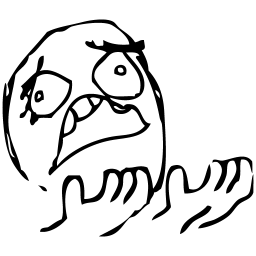
\includegraphics[height=5cm]{images/whyyy.png}
\end{center}

Why did we learn this?
\end{frame}

\section{Functor}
\label{sec:org4d3b868}
\begin{frame}[label={sec:org924285c}]{Function Application}
\alert{Function} is one of the most important pillars of the functional programming.
Naturally, we can manipulate functions in two ways:

\begin{enumerate}
\item Create function (abstraction).
\item Apply function to an argument (application).
\end{enumerate}
\end{frame}

\begin{frame}[label={sec:orgc963c6c},fragile]{Function Application}
 We know how to apply functions.

\begin{minted}[]{scala}
def inc: Int => Int = v => v + 1
def add: Int => Int => Int = a => b => a + b

inc(42)      // => 43
add(100)     // => function of type Int => Int
add(100)(42) // => 142
\end{minted}

\pause

We can define a special function that will apply first argument to second.

\begin{minted}[]{scala}
def apply[A, B]: (A => B) => A => B =
  f => v => f(v)

apply(inc)(42)      // => 43
apply(add)(100)     // => function of type Int => Int
apply(add)(100)(42) // => 142
\end{minted}
\end{frame}

\begin{frame}[label={sec:orge2647ce},fragile]{Function Application}
 While this doesn't seem to be useful, it's important to understand type
signature of \texttt{apply} function:

\begin{minted}[]{scala}
apply :   (A => B)    => A        => B
//        function    argument    result
\end{minted}

\pause

It's higher-order function.
\end{frame}

\begin{frame}[label={sec:orgbed89dd},fragile]{Context: optional value}
 \texttt{Option} (or \texttt{Maybe}) is used to represent a context of value that may be
absent.

\begin{columns}
\begin{column}[t]{0.5\columnwidth}
\begin{minted}[]{scala}
trait Option[+A]
case object None extends Option[Nothing]
case class Some[+A](value: A) extends Option[A]
\end{minted}
\end{column}

\begin{column}[t]{0.5\columnwidth}
\begin{minted}[]{haskell}
data Maybe a = Nothing | Just a
\end{minted}
\end{column}
\end{columns}

\texttt{Option} is unary type constructor with kind \(* \rightarrow *\).
\end{frame}

\begin{frame}[label={sec:orgfb69fb3},fragile]{Context: optional value}
 \begin{itemize}
\item \texttt{Option(42)} is a value of type \texttt{Option[Int]}.
\item \texttt{apply} can't be used to apply \texttt{inc} to \texttt{42} in that context.
\begin{minted}[]{scala}
apply: (A => B) => A => B
inc: Int => Int
apply(inc)(Option(42))
  type mismatch;
   found   : Option[Int]
   required: Int
\end{minted}
\item <2-> But we can define custom \texttt{apply} function.
\end{itemize}
\end{frame}

\begin{frame}[label={sec:orge5e66c3},fragile]{Context: optional value}
 \begin{minted}[]{scala}
//  apply        : (A => B) =>        A  =>        B
def applyToOption: (A => B) => Option[A] => Option[B] = f => maybeV => maybeV match {
  case None    => None
  case Some(v) => Some(f(v))
}

applyToOption(inc)(Some(42))            // => Some(43)
applyToOption(inc)(None)                // => None
\end{minted}
\end{frame}

\begin{frame}[label={sec:org4d5ceb5},fragile]{Many contexts}
 \begin{itemize}
\item \texttt{Either} - a context of values with two possibilities. We mostly use it as a
context of a value that may be absent with some reason (error).
\item \texttt{List} - a context of non-deterministic choice.
\item \texttt{Future} - a context of value that is not yet computed.
\item \texttt{WIO} - a context of value with some possible side-effect.
\item \ldots{}
\end{itemize}
\end{frame}

\begin{frame}[label={sec:org1f7ab80},fragile]{Many applies}
 \begin{minted}[]{scala}
def apply           : (A => B) =>        A  =>        B
def applyToOption   : (A => B) => Option[A] => Option[B]
def applyToFuture   : (A => B) => Future[A] => Future[B]
def applyToWIO      : (A => B) =>    WIO[A] =>    WIO[B]
\end{minted}

\pause

\begin{minted}[]{scala}
def applyToContext  : (A => B) =>      F[A] =>      F[B]
\end{minted}
\end{frame}

\begin{frame}[label={sec:orgf430649}]{Repetition is}
\begin{center}
\includegraphics[height=5cm]{images/cucumber.jpg}
\end{center}

Cucumbersome
\end{frame}

\begin{frame}[label={sec:org8d59480},fragile]{Functoriana}
 \begin{minted}[]{scala}
trait Functor[F[_]] {
  def fmap[A, B]: (A => B) => F[A] => F[B]
}
\end{minted}

\pause

\begin{minted}[]{scala}
object OptionImpl {
  implicit val optionFunctor: Functor[Option] = {
    def fmap[A, B]: (A => B) => Option[A] => Option[B] =
      f => fa => fa match {
        case None    => None
        case Some(v) => Some(f(v))
      }
  }
}
\end{minted}
\end{frame}

\begin{frame}[label={sec:org78c4f0a},fragile]{Code responsibly, know the laws}
 \begin{enumerate}
\item <1-> \texttt{fmap id = id}
\item <2-> \texttt{fmap (g . f) = fmap g . fmap f}
\item <3-> Functor doesn't change the context nor it's shape.
\begin{enumerate}
\item \texttt{Option} - failure to failure, success to success
\item \texttt{List} - length is unchanged
\item Value constructor defines the shape.
\end{enumerate}
\end{enumerate}
\end{frame}

\begin{frame}[label={sec:orgcc361cc}]{Sum type: Option}
\begin{center}
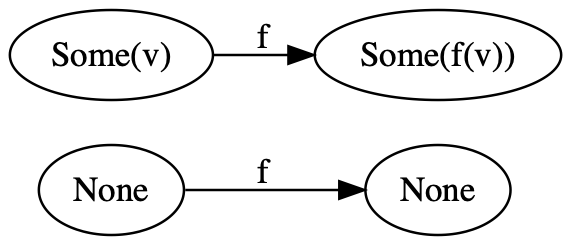
\includegraphics[height=3.5cm]{.dot/functor-option.png}
\end{center}

\begin{itemize}
\item Failure to failure.
\item Success to success.
\item Shape is unchanged.
\item Constructor is not changed.
\end{itemize}
\end{frame}

\begin{frame}[label={sec:org60efde3},fragile]{Breaking the Option}
 \begin{minted}[]{scala}
  fmap(identity)(value)
= identity(value)
= value
\end{minted}

\pause

\begin{minted}[]{scala}
implicit val optionFunctor: Functor[Option] = {
  def fmap[A, B]: (A => B) => Option[A] => Option[B] =
    f => fa => fa match {
      case None    => None
      case Some(v) => None
    }
}
\end{minted}

\pause

\begin{minted}[]{scala}
  fmap(identity)(None)
= None == None

  fmap(indentity)(Some(42))
= None != Some(42)
\end{minted}

Shape is destroyed!
\end{frame}

\begin{frame}[label={sec:orgefd37c4},fragile]{Product type: List}
 \begin{columns}
\begin{column}[t]{0.5\columnwidth}
\begin{center}
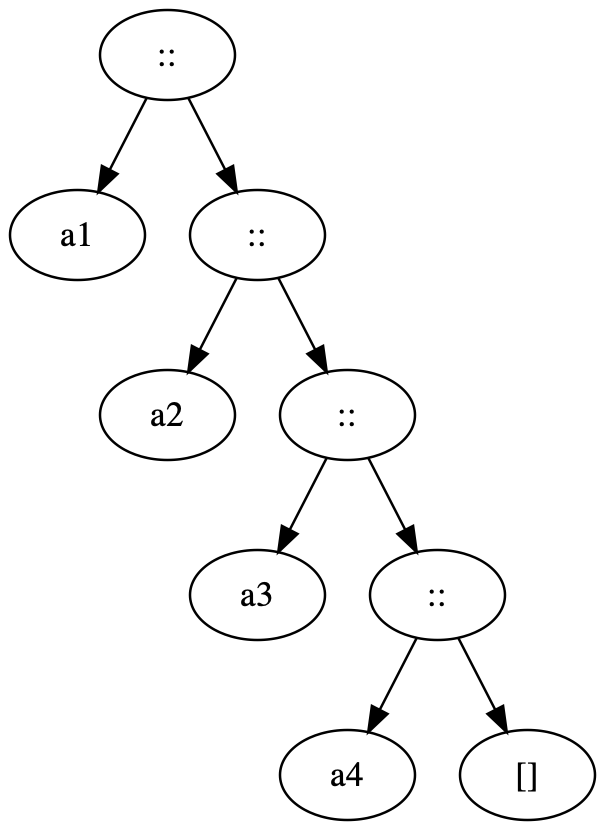
\includegraphics[height=4.5cm]{.dot/functor-list-1.png}
\end{center}
\end{column}

\begin{column}[t]{0.5\columnwidth}
\begin{center}
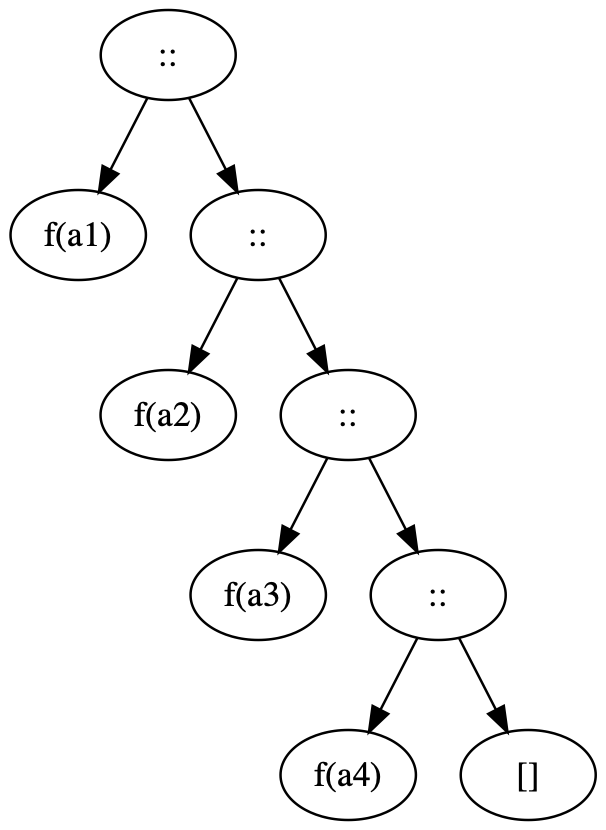
\includegraphics[height=4.5cm]{.dot/functor-list-2.png}
\end{center}
\end{column}
\end{columns}

\begin{itemize}
\item Shape is unchanged.
\item Length remains the same.
\item Spine remains the same.
\item Length is amount of \texttt{::} constructors.
\end{itemize}
\end{frame}

\begin{frame}[label={sec:org25afb68},fragile,t]{Breaking the List}
 \begin{onlyenv}<1-2>
\begin{minted}[]{scala}
implicit val listFunctor: Functor[List] = new Functor[List] {
  override def fmap[A, B](f: A => B)(fa: List[A]): List[B] = fa match {
    case Nil => Nil
    case x :: xs => f(x) :: f(x) :: fmap(f)(xs)
    //              ^ extra concatenation
  }
}
\end{minted}
\end{onlyenv}

\begin{onlyenv}<2-3>
\begin{minted}[]{scala}
  fmap(identity)(List(a, b))
= identity(a) :: identity(a) :: identity(b) :: identity(b) :: Nil
= a :: a :: b :: b :: Nil
= List(a, a, b, b) != List(a, b)
\end{minted}
\end{onlyenv}

\begin{onlyenv}<3>
Shape is destroyed!

\begin{columns}
\begin{column}[t]{0.5\columnwidth}
\begin{center}
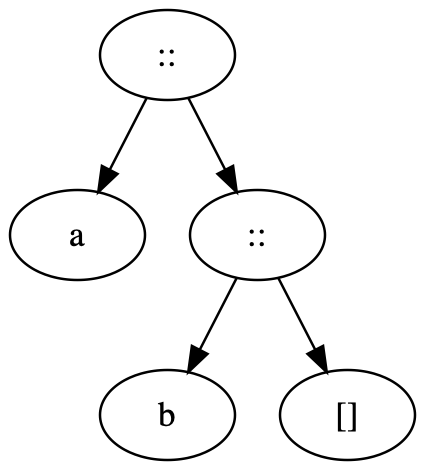
\includegraphics[height=4.5cm]{.dot/functor-list-broken-1.png}
\end{center}
\end{column}

\begin{column}[t]{0.5\columnwidth}
\begin{center}
\includegraphics[height=4.5cm]{.dot/functor-list-broken-2.png}
\end{center}
\end{column}
\end{columns}
\end{onlyenv}
\end{frame}

\begin{frame}[label={sec:org9ca7985}]{What about the second rule?}
As a result of the Free Theorem (Wadler), it's impossible to break the second
rule in Haskell without breaking the first one.

If you are interested in details, let's talk after the forkshop.

\begin{itemize}
\item \url{https://ttic.uchicago.edu/\~dreyer/course/papers/wadler.pdf}
\item \url{https://www.schoolofhaskell.com/user/edwardk/snippets/fmap}
\end{itemize}
\end{frame}

\begin{frame}[label={sec:orgb19477b}]{There can be only one}
There is only one lawful implementation of Functor for a given type.
\end{frame}

\begin{frame}[label={sec:org512d344},fragile]{Coding time}
 \begin{itemize}
\item Open \texttt{src/main/scala/wax/typeclass/functor/implicits/package.scala} file.
\item Task is to add missing implementations (no \texttt{???}).
\item Run \texttt{FunctorSpec} to test your implementation.
\end{itemize}
\end{frame}

\begin{frame}[label={sec:org0a8d9cb},fragile]{Outcome}
 \begin{itemize}
\item Function application is very important.
\item \texttt{Functor} provides us with means to apply regular function to value in a
context, without changing the shape of the context.
\item Laws make it impossible to provide multiple different functor instances.
\item Do you dare to dream of something more?
\begin{itemize}
\item <2-> (hopefully yes)
\end{itemize}
\end{itemize}
\end{frame}

\section{Applicative Functor}
\label{sec:org83d8649}

\begin{frame}[label={sec:org7121261},fragile]{Next step}
 \begin{minted}[]{scala}
val v1 = Option(42)
val v2 = Option(100)

def add: Int => Int => Int =
  a => b => a + b
// add: Int => (Int => Int)
\end{minted}

\pause

\begin{minted}[]{scala}
val result = v1.fmap(add)
// result: Option[Int => Int]
\end{minted}

\pause

Now we have:

\begin{itemize}
\item \texttt{result} of type \texttt{Option[Int => Int]}
\item \texttt{v2} of type \texttt{Option[Int]}
\end{itemize}

And we want to apply that function and get resulting \texttt{Option[Int]}.
\end{frame}

\begin{frame}[label={sec:orgdac5edd},fragile]{Next step}
 \begin{minted}[]{scala}
def apply :  (A => B) =>   A  =>   B
def fmap  :  (A => B) => F[A] => F[B]
\end{minted}

\pause

\begin{minted}[]{scala}
def ???   : F[A => B] => F[A] => F[B]
\end{minted}
\end{frame}

\begin{frame}[label={sec:org9e5cb40},fragile]{Solution}
 \begin{minted}[]{scala}
val v1 = Option(42)
val v2 = Option(100)

def applyOptionF[A, B]: Option[A => B] => Option[A] => Option[B] =
  ff => fv => ff match {
    case None    => None
    case Some(f) => fv.fmap(f)
  }

applyOptionF(v1.fmap(add))(v2)
\end{minted}
\end{frame}

\begin{frame}[label={sec:orga0882fa},fragile]{Following the same idea}
 \begin{minted}[]{scala}
trait Applicative[F[_]] extends Functor[F] {
  def ap[A, B]: F[A => B] => F[A] => F[B]

  def pure[A](a: A): A => F[A]
}
\end{minted}

\pause

\begin{columns}
\begin{column}[t]{0.46\columnwidth}
\begin{minted}[]{scala}
v1.fmap(add).ap(v2)
// v1 `add` v2
// <*> = ap
\end{minted}

\pause
\end{column}

\begin{column}[t]{0.46\columnwidth}
\begin{minted}[]{haskell}
f <$> v1 <*> v2
-- much like a simple function application
-- f v1 v2
\end{minted}
\end{column}
\end{columns}
\end{frame}

\begin{frame}[label={sec:orgb623a25},fragile]{What's about pure?}
 \begin{columns}
\begin{column}[t]{0.4\columnwidth}
\begin{minted}[]{scala}
trait Functor[F[_]] {
  def fmap[A, B]: (A => B) => F[A] => F[B]
}
\end{minted}
\end{column}

\begin{column}[t]{0.4\columnwidth}
\begin{minted}[]{scala}
trait Applicative[F[_]] extends Functor[F] {
  def ap[A, B]: F[A => B] => F[A] => F[B]

  def pure[A](a: A): A => F[A]
}
\end{minted}
\end{column}
\end{columns}

\begin{enumerate}
\item <1-> It abstracts the value constructor.
\item <2-> By itself it doesn't have much importance without \texttt{ap}.
\item <3-> Important for \texttt{Applicative} laws.
\item <4-> Ties \texttt{Functor} and \texttt{Applicative}.
\begin{itemize}
\item \texttt{fmap(f)(x) == ap(pure(f))(x)}
\item \texttt{fmap f x = pure f <*> x}
\end{itemize}
\item <5-> Useful in practice.
\end{enumerate}
\end{frame}

\begin{frame}[label={sec:orgeb67c16},fragile]{Another perspective}
 \texttt{Applicative} interface is useful in day-to-day development.

\pause

\texttt{Applicative} has equivalent type class \texttt{Monoidal} functor:

\begin{columns}
\begin{column}[t]{0.5\columnwidth}
\begin{minted}[]{scala}
trait Applicative[F[_]] extends Functor[F] {
  def pure[A](a: A): F[A]
  def ap[A, B](f: F[A => B])(fa: F[A]): F[B]
}
\end{minted}
\end{column}

\begin{column}[t]{0.5\columnwidth}
\begin{minted}[]{scala}
trait Monoidal[F[_]] extends Functor[F] {
  def unit: F[Unit]
  def comb[A, B](fa: F[A], fb: F[B]): F[(A, B)]
}
\end{minted}
\end{column}
\end{columns}
\end{frame}

\begin{frame}[label={sec:org4280814},fragile]{From \texttt{Applicative} to \texttt{Monoidal}}
 \begin{columns}
\begin{column}[t]{0.5\columnwidth}
\begin{minted}[]{scala}
trait Applicative[F[_]] extends Functor[F] {
  def pure[A](a: A): F[A]
  def ap[A, B](f: F[A => B])(fa: F[A]): F[B]
}
\end{minted}
\end{column}

\begin{column}[t]{0.5\columnwidth}
\begin{minted}[]{scala}
trait Monoidal[F[_]] extends Functor[F] {
  def unit: F[Unit]
  def comb[A, B](fa: F[A], fb: F[B]): F[(A, B)]
}
\end{minted}
\end{column}
\end{columns}

\begin{minted}[]{scala}
class ApplicativeToMonoida[F[_]: Applicative]() extends Monoidal[F] {
  override def unit: F[Unit] = ???

  override def comb[A, B](fa: F[A], fb: F[B]): F[(A, B)] = ???
}
\end{minted}
\end{frame}

\begin{frame}[label={sec:orgefc79ad},fragile]{From \texttt{Applicative} to \texttt{Monoidal}}
 \begin{columns}
\begin{column}[t]{0.5\columnwidth}
\begin{minted}[]{scala}
trait Applicative[F[_]] extends Functor[F] {
  def pure[A](a: A): F[A]
  def ap[A, B](f: F[A => B])(fa: F[A]): F[B]
}
\end{minted}
\end{column}

\begin{column}[t]{0.5\columnwidth}
\begin{minted}[]{scala}
trait Monoidal[F[_]] extends Functor[F] {
  def unit: F[Unit]
  def comb[A, B](fa: F[A], fb: F[B]): F[(A, B)]
}
\end{minted}
\end{column}
\end{columns}

\begin{minted}[]{scala}
class ApplicativeToMonoida[F[_]: Applicative]() extends Monoidal[F] {
  override def unit: F[Unit] = Applicative[F].pure(())

  override def comb[A, B](fa: F[A], fb: F[B]): F[(A, B)] = ???
}
\end{minted}
\end{frame}

\begin{frame}[label={sec:org0348b1c},fragile]{From \texttt{Applicative} to \texttt{Monoidal}}
 \begin{columns}
\begin{column}[t]{0.5\columnwidth}
\begin{minted}[]{scala}
trait Applicative[F[_]] extends Functor[F] {
  def pure[A](a: A): F[A]
  def ap[A, B](f: F[A => B])(fa: F[A]): F[B]
}
\end{minted}
\end{column}

\begin{column}[t]{0.5\columnwidth}
\begin{minted}[]{scala}
trait Monoidal[F[_]] extends Functor[F] {
  def unit: F[Unit]
  def comb[A, B](fa: F[A], fb: F[B]): F[(A, B)]
}
\end{minted}
\end{column}
\end{columns}

\begin{minted}[]{scala}
class ApplicativeToMonoida[F[_]: Applicative]() extends Monoidal[F] {
  override def unit: F[Unit] = Applicative[F].pure(())

  override def comb[A, B](fa: F[A], fb: F[B]): F[(A, B)] =
    fa.fmap((a: A) => (b: B) => (a, b)).ap(fb)
}
\end{minted}
\end{frame}

\begin{frame}[label={sec:orgdf0b462},fragile]{From \texttt{Monoidal} to \texttt{Applicative}}
 \begin{columns}
\begin{column}[t]{0.5\columnwidth}
\begin{minted}[]{scala}
trait Applicative[F[_]] extends Functor[F] {
  def pure[A](a: A): F[A]
  def ap[A, B](f: F[A => B])(fa: F[A]): F[B]
}
\end{minted}
\end{column}

\begin{column}[t]{0.5\columnwidth}
\begin{minted}[]{scala}
trait Monoidal[F[_]] extends Functor[F] {
  def unit: F[Unit]
  def comb[A, B](fa: F[A], fb: F[B]): F[(A, B)]
}
\end{minted}
\end{column}
\end{columns}

\begin{minted}[]{scala}
class MonoidalToApplicative[F[_]: Monoidal]() extends Applicative[F] {
  override def pure[A](a: A): F[A] = ???

  override def ap[A, B](ff: F[A => B])(fa: F[A]): F[B] = ???
}
\end{minted}
\end{frame}

\begin{frame}[label={sec:org44a95ae},fragile]{From \texttt{Monoidal} to \texttt{Applicative}}
 \begin{columns}
\begin{column}[t]{0.5\columnwidth}
\begin{minted}[]{scala}
trait Applicative[F[_]] extends Functor[F] {
  def pure[A](a: A): F[A]
  def ap[A, B](f: F[A => B])(fa: F[A]): F[B]
}
\end{minted}
\end{column}

\begin{column}[t]{0.5\columnwidth}
\begin{minted}[]{scala}
trait Monoidal[F[_]] extends Functor[F] {
  def unit: F[Unit]
  def comb[A, B](fa: F[A], fb: F[B]): F[(A, B)]
}
\end{minted}
\end{column}
\end{columns}

\begin{minted}[]{scala}
class MonoidalToApplicative[F[_]: Monoidal]() extends Applicative[F] {
  override def pure[A](a: A): F[A] = Monoidal[F].unit.fmap(_ => a)

  override def ap[A, B](ff: F[A => B])(fa: F[A]): F[B] = ???
}
\end{minted}
\end{frame}

\begin{frame}[label={sec:org5a6b28a},fragile]{From \texttt{Monoidal} to \texttt{Applicative}}
 \begin{columns}
\begin{column}[t]{0.5\columnwidth}
\begin{minted}[]{scala}
trait Applicative[F[_]] extends Functor[F] {
  def pure[A](a: A): F[A]
  def ap[A, B](f: F[A => B])(fa: F[A]): F[B]
}
\end{minted}
\end{column}

\begin{column}[t]{0.5\columnwidth}
\begin{minted}[]{scala}
trait Monoidal[F[_]] extends Functor[F] {
  def unit: F[Unit]
  def comb[A, B](fa: F[A], fb: F[B]): F[(A, B)]
}
\end{minted}
\end{column}
\end{columns}

\begin{minted}[]{scala}
class MonoidalToApplicative[F[_]: Monoidal]() extends Applicative[F] {
  override def pure[A](a: A): F[A] = Monoidal[F].unit.fmap(_ => a)

  override def ap[A, B](ff: F[A => B])(fa: F[A]): F[B] = Monoidal[F].comb(ff, fa).fmap { case (f, a) => f(a) }
}
\end{minted}
\end{frame}

\begin{frame}[label={sec:orgf327dc9},fragile]{From \texttt{Monoidal} to \texttt{Applicative}}
 \begin{minted}[]{scala}
class MonoidalToApplicative[F[_]: Monoidal]() extends Applicative[F] {
  override def pure[A](a: A): F[A] = Monoidal[F].unit.fmap(_ => a)

  override def ap[A, B](ff: F[A => B])(fa: F[A]): F[B] = Monoidal[F].comb(ff, fa).fmap { case (f, a) => f(a) }
}
\end{minted}

Path from \texttt{Monoidal} to \texttt{Applicative} is through function application. Function
application is a practical thing.
\end{frame}

\begin{frame}[label={sec:orgcd54b47},fragile]{Some symmetry}
 \begin{minted}[]{scala}
def ap:   F[ A =>  B]  => (F[A] => F[B])
def comb: (F[A], F[B]) => F[(A,      B)]
\end{minted}
\end{frame}

\begin{frame}[label={sec:orge79e476},fragile]{Monoid part of \texttt{Monoidal}}
 \begin{columns}
\begin{column}[t]{0.5\columnwidth}
\begin{minted}[]{scala}
trait Monoid[A] {
  def empty: A
  def combine(x: A, y: A): A
}
\end{minted}
\end{column}

\begin{column}[t]{0.5\columnwidth}
\begin{minted}[]{scala}
trait Monoidal[F[_]] extends Functor[F] {
  def unit: F[Unit]
  def comb[A, B](fa: F[A], fb: F[B]): F[(A, B)]
}
\end{minted}
\end{column}
\end{columns}

\begin{itemize}
\item <2-> \texttt{Monoidal} is \texttt{Monoid} for \texttt{Functors}.
\item <3-> \texttt{Applicative} is \texttt{Monoidal}.
\item <4-> \texttt{Applicative} is \texttt{Monoid} for \texttt{Functors}.
\end{itemize}
\end{frame}

\begin{frame}[label={sec:org13321b8},fragile]{Applicative laws}
 \begin{enumerate}
\item Identity: \texttt{pure id <*> v = v}
\begin{itemize}
\item Identity in context does nothing. Like regular identity.
\end{itemize}
\item Homomorphism: \texttt{pure f <*> pure x = pure (f x)}
\begin{itemize}
\item \texttt{pure} preserves function application.
\end{itemize}
\item Interchange: \texttt{u <*> pure y = pure (\$ y) <*> u}
\begin{itemize}
\item Applying function in a context to a value in a context is the same as
applying a pure function of argument application to a function in a context.
\item Don't think to much about this.
\end{itemize}
\item Composition: \texttt{pure (.) <*> u <*> v <*> w = u <*> (v <*> w)}
\begin{itemize}
\item Says that function composition 'holds' in the applicative context.
\end{itemize}
\end{enumerate}
\end{frame}

\begin{frame}[label={sec:orge2c76b0},fragile]{Monoidal laws}
 \begin{enumerate}
\item Left identity: \texttt{comb (u, unit) \textasciitilde{} u}
\item Right identity: \texttt{comb (unit, u) \textasciitilde{} u}
\item Associativity: \texttt{comb (comb (u, v), w) \textasciitilde{} comb (u, comb (v, w))}
\end{enumerate}
\end{frame}

\begin{frame}[label={sec:org5790ebe},fragile]{Coding time}
 \begin{itemize}
\item Open \texttt{src/main/scala/wax/typeclass/applicative/implicits/package.scala}
\item Task is to add missing implementations (no \texttt{???}).
\item Run \texttt{ApplicativeSpec} to test your implementation.
\end{itemize}
\end{frame}

\begin{frame}[label={sec:org44f6352},fragile]{Conditionals}
 \begin{minted}[]{scala}
def iffy[F[_]: Applicative, A](fb: F[Boolean], ft: F[A], fe: F[A]): F[A] = {
  def cond: Boolean => A => A => A = b => t => e => if (b) t else e
  Applicative[F].pure(cond).ap(fb).ap(ft).ap(fe)
}
\end{minted}

\pause

\begin{minted}[]{scala}
> iffy(Option(true), Option(42), Option(100))
\end{minted}

\pause

\begin{minted}[]{scala}
Some(42)
\end{minted}

\pause

\begin{minted}[]{scala}
> iffy(Option(true), Option(42), None)
\end{minted}

\pause

\begin{minted}[]{scala}
None
\end{minted}

\pause

\begin{minted}[]{scala}
> iffy(IO(true), IO(println("true case")), IO(println("false case"))).unsafeRunSync()
\end{minted}

\pause

\begin{minted}[]{scala}
true case
false case
\end{minted}
\end{frame}

\begin{frame}[label={sec:org18c261b},fragile]{Outcome}
 \begin{itemize}
\item <1-> \texttt{Monoid} and \texttt{Functor} are two fundamental objects.
\item <2-> We can apply regular function to multiple values in context.
\item <3-> With applicatives, computations have a fixed unconditional structure.
\end{itemize}
\end{frame}

\section{Parsing}
\label{sec:org594ab0d}

\begin{frame}[label={sec:org503ac12},fragile,t]{Parsing}
 \vspace*{20px}

Parsing is the process of transforming input data (frequently text) to data
structure.

\begin{onlyenv}<2->
\begin{minted}[]{scala}
case class Parser[A](parse: String => ParserResult[A])
\end{minted}
\end{onlyenv}

\begin{onlyenv}<3->
\begin{minted}[]{scala}
sealed trait ParserResult[A]
case class ParserFailure[A]() extends ParserResult[A]
case class ParserSuccess[A](value: A, remainder: String) extends ParserResult[A]
\end{minted}

\pause
\end{onlyenv}

\begin{onlyenv}<4>
\begin{minted}[]{scala}
def run[A](parser: Parser[A])(input: String): Either[String, A] = parser.parse(input) match {
  case ParserFailure()                   => Left("parser error")


}
\end{minted}
\end{onlyenv}

\begin{onlyenv}<5>
\begin{minted}[]{scala}
def run[A](parser: Parser[A])(input: String): Either[String, A] = parser.parse(input) match {
  case ParserFailure()                   => Left("parser error")
  case ParserSuccess(_, s) if s.nonEmpty => Left("parser did not consume entire stream: '" ++ s ++ "'")

}
\end{minted}
\end{onlyenv}

\begin{onlyenv}<6>
\begin{minted}[]{scala}
def run[A](parser: Parser[A])(input: String): Either[String, A] = parser.parse(input) match {
  case ParserFailure()                   => Left("parser error")
  case ParserSuccess(_, s) if s.nonEmpty => Left("parser did not consume entire stream: '" ++ s ++ "'")
  case ParserSuccess(v, _)               => Right(v)
}
\end{minted}
\end{onlyenv}
\end{frame}

\begin{frame}[label={sec:org28a2bbe},fragile,t]{Simple parser}
 \begin{minted}[]{scala}
case class Parser[A](parse: String => ParserResult[A])
\end{minted}

\begin{columns}
\begin{column}[t]{0.5\columnwidth}
\begin{onlyenv}<1>
\begin{minted}[]{scala}
def char(c: Char): Parser[Char] = Parser { s =>
  ???
}
\end{minted}
\end{onlyenv}

\begin{onlyenv}<2>
\begin{minted}[]{scala}
def char(c: Char): Parser[Char] = Parser { s =>
  if (s.isEmpty) ???
  else ???
}
\end{minted}
\end{onlyenv}

\begin{onlyenv}<3-4>
\begin{minted}[]{scala}
def char(c: Char): Parser[Char] = Parser { s =>
  if (s.isEmpty) ParserFailure()
  else ???
}
\end{minted}
\end{onlyenv}

\begin{onlyenv}<5>
\begin{minted}[]{scala}
def char(c: Char): Parser[Char] = Parser { s =>
  if (s.isEmpty) ParserFailure()
  else if (s.head != c) ???
  else ???
}
\end{minted}
\end{onlyenv}

\begin{onlyenv}<6-7>
\begin{minted}[]{scala}
def char(c: Char): Parser[Char] = Parser { s =>
  if (s.isEmpty) ParserFailure()
  else if (s.head != c) ParserFailure()
  else ???
}
\end{minted}
\end{onlyenv}

\begin{onlyenv}<8->
\begin{minted}[]{scala}
def char(c: Char): Parser[Char] = Parser { s =>
  if (s.isEmpty) ParserFailure()
  else if (s.head != c) ParserFailure()
  else ParserSuccess(s.head,        s.tail)
  //                 ^ parsed char  ^ remaining stream
}
\end{minted}
\end{onlyenv}
\end{column}

\begin{column}[t]{0.5\columnwidth}
\begin{onlyenv}<4->
\begin{minted}[]{scala}
> char('c').run("")
Left("parse error")
\end{minted}
\end{onlyenv}

\begin{onlyenv}<7->
\begin{minted}[]{scala}
> char('c').run("C")
Left("parse error")
\end{minted}
\end{onlyenv}

\begin{onlyenv}<9->
\begin{minted}[]{scala}
> char('c').run("c")
Right('c')
\end{minted}
\end{onlyenv}

\begin{onlyenv}<10->
\begin{minted}[]{scala}
> char('c').run("comelette")
Left("parser did not consume entire stream: 'omelette'")
\end{minted}
\end{onlyenv}

\begin{onlyenv}<11->
\begin{center}
\includegraphics[height=3cm]{images/omelette.jpg}
\end{center}
\end{onlyenv}
\end{column}
\end{columns}
\end{frame}

\begin{frame}[label={sec:orge01e743},fragile]{Abstracting \texttt{char}}
 \begin{minted}[]{scala}
def satisfy(pred: Char => Boolean): Parser[Char] = Parser { s =>
  if (s.nonEmpty && pred(s.head)) ParserSuccess(s.head, s.tail)
  else ParserFailure()
}
\end{minted}

\pause

\begin{minted}[]{scala}
def char(a: Char): Parser[Char] = satisfy(_ == a)

def notChar(a: Char): Parser[Char] = satisfy(_ != a)

def anyChar: Parser[Char] = satisfy(_ => true)

def space: Parser[Char] = char(' ')
\end{minted}
\end{frame}

\begin{frame}[label={sec:org1fe7761},fragile,t]{Repeating the parser}
 \begin{onlyenv}<1>
\begin{minted}[]{scala}
def many[A](parser: Parser[A]): Parser[List[A]] = Parser { s =>
  ???
}
\end{minted}
\end{onlyenv}

\begin{onlyenv}<2>
\begin{minted}[]{scala}
def many[A](parser: Parser[A]): Parser[List[A]] = Parser { s =>
  parser.parse(s) match {
    case ParserSuccess(v, s1) => ???
    case ParserFailure()      => ???
  }
}
\end{minted}
\end{onlyenv}

\begin{onlyenv}<3>
\begin{minted}[]{scala}
def many[A](parser: Parser[A]): Parser[List[A]] = Parser { s =>
  parser.parse(s) match {
    case ParserSuccess(v, s1) =>
      many(parser)           // recursivelly create a Parser[List[A]]

    case ParserFailure()      => ???
  }
}
\end{minted}
\end{onlyenv}

\begin{onlyenv}<4>
\begin{minted}[]{scala}
def many[A](parser: Parser[A]): Parser[List[A]] = Parser { s =>
  parser.parse(s) match {
    case ParserSuccess(v, s1) =>
      many(parser)           // recursivelly create a Parser[List[A]]
        .parse(s1)           // run it on the remaining stream to get ParserResult[List[A]]

    case ParserFailure()      => ???
  }
}
\end{minted}
\end{onlyenv}

\begin{onlyenv}<5>
\begin{minted}[]{scala}
def many[A](parser: Parser[A]): Parser[List[A]] = Parser { s =>
  parser.parse(s) match {
    case ParserSuccess(v, s1) =>
      many(parser)           // recursivelly create a Parser[List[A]]
        .parse(s1)           // run it on the remaining stream to get ParserResult[List[A]]
        .fmap(xs => v :: xs) // append parsed value to the list

    case ParserFailure()      => ???
  }
}
\end{minted}
\end{onlyenv}

\begin{onlyenv}<6>
\begin{minted}[]{scala}
def many[A](parser: Parser[A]): Parser[List[A]] = Parser { s =>
  parser.parse(s) match {
    case ParserSuccess(v, s1) =>
      many(parser)           // recursivelly create a Parser[List[A]]
        .parse(s1)           // run it on the remaining stream to get ParserResult[List[A]]
        .fmap(xs => v :: xs) // append parsed value to the list

    case ParserFailure()      => ParserSuccess(List.empty, s)
    // We can't return Failure, otherwise whole parser will fail
  }
}
\end{minted}
\end{onlyenv}
\end{frame}

\begin{frame}[label={sec:org46a905c},fragile,t]{Repeating the parser}
 \begin{onlyenv}<1>
\begin{minted}[]{scala}
many(satisfy(_.isLetter)).parse("brânză")
\end{minted}
\end{onlyenv}

\begin{onlyenv}<2>
\begin{minted}[]{scala}
satisfy(_.isLetter).parse("brânză") match {
  case ParserSuccess(v, s1) =>
    many(satisfy(_.isLetter)).parse(s1).fmap(xs => v :: xs)
  case ParserFailure() => ParserSuccess(List.empty, s)
}
\end{minted}
\end{onlyenv}

\begin{onlyenv}<3>
\begin{minted}[]{scala}
case ParserSuccess('b', "rânză") match {
  case ParserSuccess(v, s1) =>
    many(satisfy(_.isLetter)).parse(s1).fmap(xs => v :: xs)
  case ParserFailure() => ParserSuccess(List.empty, s)
}
\end{minted}
\end{onlyenv}

\begin{onlyenv}<4>
\begin{minted}[]{scala}
many(satisfy(_.isLetter)).parse("rânză")
  .fmap(xs => 'b' :: xs)
\end{minted}
\end{onlyenv}

\begin{onlyenv}<5>
\begin{minted}[]{scala}
val res = satisfy(_.isLetter).parse("rânză") match {
  case ParserSuccess(v, s1) =>
    many(satisfy(_.isLetter)).parse(s1).fmap(xs => v :: xs)
  case ParserFailure() => ParserSuccess(List.empty, s)
}

res.fmap(xs => 'b' :: xs)
\end{minted}
\end{onlyenv}

\begin{onlyenv}<6>
\begin{minted}[]{scala}
val res = ParserSuccess('r', "ânză") match {
  case ParserSuccess(v, s1) =>
    many(satisfy(_.isLetter)).parse(s1).fmap(xs => v :: xs)
  case ParserFailure() => ParserSuccess(List.empty, s)
}

res.fmap(xs => 'b' :: xs)
\end{minted}
\end{onlyenv}

\begin{onlyenv}<7>
\begin{minted}[]{scala}
val res = many(satisfy(_.isLetter)).parse("ânză").fmap(xs => 'r' :: xs)
res.fmap(xs => 'b' :: xs)
\end{minted}
\end{onlyenv}

\begin{onlyenv}<8>
\begin{minted}[]{scala}
many(satisfy(_.isLetter)).parse("ânză")
  .fmap(xs => 'r' :: xs)
  .fmap(xs => 'b' :: xs)
\end{minted}
\end{onlyenv}

\begin{onlyenv}<9>
\begin{center}
\includegraphics[width=.9\linewidth]{images/one-eternity-later.jpg}
\end{center}
\end{onlyenv}

\begin{onlyenv}<10>
\begin{minted}[]{scala}
many(satisfy(_.isLetter)).parse("")
  .fmap(xs => 'ă' :: xs)
  .fmap(xs => 'z' :: xs)
  .fmap(xs => 'n' :: xs)
  .fmap(xs => 'â' :: xs)
  .fmap(xs => 'r' :: xs)
  .fmap(xs => 'b' :: xs)
\end{minted}
\end{onlyenv}

\begin{onlyenv}<11>
\begin{minted}[]{scala}
val res = satisfy(_.isLetter).parse("") match {
  case ParserSuccess(v, s1) =>
    many(satisfy(_.isLetter)).parse(s1).fmap(xs => v :: xs)
  case ParserFailure() => ParserSuccess(List.empty, s)
}


res
  .fmap(xs => 'ă' :: xs)
  .fmap(xs => 'z' :: xs)
  .fmap(xs => 'n' :: xs)
  .fmap(xs => 'â' :: xs)
  .fmap(xs => 'r' :: xs)
  .fmap(xs => 'b' :: xs)
\end{minted}
\end{onlyenv}

\begin{onlyenv}<12>
\begin{minted}[]{scala}
val res = ParserFailure() match {
  case ParserSuccess(v, s1) =>
    many(satisfy(_.isLetter)).parse(s1).fmap(xs => v :: xs)
  case ParserFailure() => ParserSuccess(List.empty, s)
}


res
  .fmap(xs => 'ă' :: xs)
  .fmap(xs => 'z' :: xs)
  .fmap(xs => 'n' :: xs)
  .fmap(xs => 'â' :: xs)
  .fmap(xs => 'r' :: xs)
  .fmap(xs => 'b' :: xs)
\end{minted}
\end{onlyenv}

\begin{onlyenv}<13>
\begin{minted}[]{scala}
val res = ParserSuccess(List.empty, "")

res
  .fmap(xs => 'ă' :: xs)
  .fmap(xs => 'z' :: xs)
  .fmap(xs => 'n' :: xs)
  .fmap(xs => 'â' :: xs)
  .fmap(xs => 'r' :: xs)
  .fmap(xs => 'b' :: xs)
\end{minted}
\end{onlyenv}

\begin{onlyenv}<14>
\begin{minted}[]{scala}
ParserSuccess(List.empty, "")
  .fmap(xs => 'ă' :: xs)
  .fmap(xs => 'z' :: xs)
  .fmap(xs => 'n' :: xs)
  .fmap(xs => 'â' :: xs)
  .fmap(xs => 'r' :: xs)
  .fmap(xs => 'b' :: xs)
\end{minted}
\end{onlyenv}

\begin{onlyenv}<15>
\begin{minted}[]{scala}
ParserSuccess(List('ă'), "")
  .fmap(xs => 'z' :: xs)
  .fmap(xs => 'n' :: xs)
  .fmap(xs => 'â' :: xs)
  .fmap(xs => 'r' :: xs)
  .fmap(xs => 'b' :: xs)
\end{minted}
\end{onlyenv}

\begin{onlyenv}<16>
\begin{minted}[]{scala}
ParserSuccess(List('z', 'ă'), "")
  .fmap(xs => 'n' :: xs)
  .fmap(xs => 'â' :: xs)
  .fmap(xs => 'r' :: xs)
  .fmap(xs => 'b' :: xs)
\end{minted}
\end{onlyenv}

\begin{onlyenv}<17>
\begin{center}
\includegraphics[width=.9\linewidth]{images/one-eternity-later.jpg}
\end{center}
\end{onlyenv}

\begin{onlyenv}<18>
\begin{minted}[]{scala}
ParserSuccess(List('b', 'r', 'â', 'n', 'z', 'ă'), "")
\end{minted}
\end{onlyenv}
\end{frame}

\begin{frame}[label={sec:org87dc180},fragile,t]{(invalid) UUID parser}
 \begin{onlyenv}<1>
\begin{minted}[]{scala}
def uuid: Parser[String] = ???
\end{minted}
\end{onlyenv}

\begin{onlyenv}<2>
\begin{minted}[]{scala}
def uuid: Parser[String] =
  satisfy(c => c.isLetterOrDigit || c == '-')
\end{minted}
\end{onlyenv}

\begin{onlyenv}<3>
\begin{minted}[]{scala}
def uuid: Parser[String] =
  satisfy(c => c.isLetterOrDigit || c == '-')
  // Required: Parser [ String ]
  // Found:    Parser [ Char   ]
\end{minted}
\end{onlyenv}

\begin{onlyenv}<4>
\begin{minted}[]{scala}
def uuid: Parser[String] =
  many(satisfy(c => c.isLetterOrDigit || c == '-'))
\end{minted}
\end{onlyenv}

\begin{onlyenv}<5>
\begin{minted}[]{scala}
def uuid: Parser[String] =
  many(satisfy(c => c.isLetterOrDigit || c == '-'))
  // Required: Parser [ String     ]
  // Found:    Parser [ List[Char] ]
\end{minted}
\end{onlyenv}

\begin{onlyenv}<6->
\begin{minted}[]{scala}
def uuid: Parser[String] =
  satisfy(c => c.isLetterOrDigit || c == '-').fmap(_.mkString)
\end{minted}
\end{onlyenv}

\begin{onlyenv}<7->
\begin{minted}[]{scala}
> uuid.run("0517b093-b49a-447a-ad66-96ac2b244859")
Right("0517b093-b49a-447a-ad66-96ac2b244859")
\end{minted}
\end{onlyenv}

\begin{onlyenv}<8->
\begin{minted}[]{scala}
> uuid.run("   0517b093-b49a-447a-ad66-96ac2b244859       ")
Left("parser error")
\end{minted}
\end{onlyenv}

\begin{onlyenv}<9->
Damn\ldots{}
\end{onlyenv}
\end{frame}

\begin{frame}[label={sec:org106b503},fragile,t]{Space invaders}
 \begin{minted}[]{scala}
def uuid: Parser[String] = /* ... */
def many[A](parser: Parser[A]): Parser[List[A]] = /* ... */
def space: Parser[Char] = /* ... */
\end{minted}

\begin{onlyenv}<1>
\begin{minted}[]{scala}
def tokenize[A](parser: Parser[A]): Parser[A] =
  ???
\end{minted}
\end{onlyenv}

\begin{onlyenv}<2>
\begin{minted}[]{scala}
def tokenize[A](parser: Parser[A]): Parser[A] =
  many(space)
\end{minted}
\end{onlyenv}

\begin{onlyenv}<3>
\begin{minted}[]{scala}
def tokenize[A](parser: Parser[A]): Parser[A] =
  many(space)
  // Required: Parser [ A          ]
  // Found:    Parser [ List[Char] ]
\end{minted}
\end{onlyenv}

\begin{onlyenv}<4>
\begin{minted}[]{scala}
def tokenize[A](parser: Parser[A]): Parser[A] =
  many(space) *> parser
\end{minted}
\end{onlyenv}

\begin{onlyenv}<5,6>
\begin{minted}[]{scala}
def tokenize[A](parser: Parser[A]): Parser[A] =
  many(space) *> parser
  // def *> : F[A] => F[B] => F[B]
\end{minted}
\end{onlyenv}

\begin{onlyenv}<6>
\begin{minted}[]{scala}
> tokenize(uuid).run("0517b093-b49a-447a-ad66-96ac2b244859")
Right("0517b093-b49a-447a-ad66-96ac2b244859")

> tokenize(uuid).run("    0517b093-b49a-447a-ad66-96ac2b244859")
Right("0517b093-b49a-447a-ad66-96ac2b244859")
\end{minted}
\end{onlyenv}

\begin{onlyenv}<7->
\begin{minted}[]{scala}
def tokenize[A](parser: Parser[A]): Parser[A] =
  many(space) *> parser <* many(space)
\end{minted}
\end{onlyenv}

\begin{onlyenv}<8>
\begin{minted}[]{scala}
> tokenize(uuid).run("             0517b093-b49a-447a-ad66-96ac2b244859 ")
Right("0517b093-b49a-447a-ad66-96ac2b244859")
\end{minted}
\end{onlyenv}
\end{frame}

\begin{frame}[label={sec:org035443c}]{So\ldots{}}
\begin{center}
\includegraphics[height=5cm]{images/applicative-confusion.jpg}
\end{center}
\end{frame}

\begin{frame}[label={sec:orga11f7db},fragile,t]{Simple case class example}
 \begin{onlyenv}<1->
\begin{minted}[]{scala}
case class Person(name: String, age: Int)
\end{minted}
\end{onlyenv}

\begin{onlyenv}<2->
\begin{minted}[]{scala}
val name: Parser[String] = some(letter).map(_.mkString)
\end{minted}
\end{onlyenv}

\begin{onlyenv}<3->
\begin{minted}[]{scala}
val int: Parser[Int] = ???
\end{minted}
\end{onlyenv}

\begin{onlyenv}<4>
\begin{minted}[]{scala}
val person: Parser[Person] =

\end{minted}
\end{onlyenv}

\begin{onlyenv}<5>
\begin{minted}[]{scala}
val person: Parser[Person] =
  name

\end{minted}
\end{onlyenv}

\begin{onlyenv}<6>
\begin{minted}[]{scala}
val person: Parser[Person] =
  name
  // Expected: Parser [ Person ]
  // Found:    Parser [ String ]
\end{minted}
\end{onlyenv}

\begin{onlyenv}<7>
\begin{minted}[]{scala}
val person: Parser[Person] =
  name.fmap(n => a => Person(n, a)).ap(int)
\end{minted}
\end{onlyenv}

\begin{onlyenv}<8,9>
\begin{columns}
\begin{column}[t]{0.5\columnwidth}
\begin{minted}[]{scala}
val person: Parser[Person] =
  name.fmap(n => a => Person(n, a)).ap(int)

val person: Parser[Person] =
  name.fmap(n => a => Person(n, a)) <*> int

val person: Parser[Person] =
  (name, int).mapN(Person)
\end{minted}
\end{column}

\begin{column}[t]{0.5\columnwidth}
\begin{minted}[]{haskell}
person :: Parser Person
person = Person <$> name <*> int

person :: Parser Person
person = liftA2 Person name int
\end{minted}
\end{column}
\end{columns}
\end{onlyenv}

\begin{onlyenv}<9>
\begin{minted}[]{scala}
> person.run("boris42")
Right(Person("boris", 42))

> person.run("boris,42")
Left("parser error")
\end{minted}

We forgot the separator!
\end{onlyenv}

\begin{onlyenv}<10->
\begin{columns}
\begin{column}[t]{0.5\columnwidth}
\begin{minted}[]{scala}
val person: Parser[Person] =
  name.fmap(n => a => Person(n, a)).ap(char ',' *> int)

val person: Parser[Person] =
  name.fmap(n => a => Person(n, a)) <*> (char ',' *> int)
\end{minted}
\end{column}

\begin{column}[t]{0.5\columnwidth}
\begin{minted}[]{haskell}
person :: Parser Person
person = Person <$> name <*> (char ',' *> int)
\end{minted}
\end{column}
\end{columns}
\end{onlyenv}

\begin{onlyenv}<11->
\begin{minted}[]{scala}
> person.run("boris,42")
Right(Person("boris", 42))
\end{minted}
\end{onlyenv}
\end{frame}

\begin{frame}[label={sec:orgfb293eb},fragile]{Coding time}
 \begin{itemize}
\item Open \texttt{src/main/scala/wax/exercise/parser/ConfigParser.scala}
\item Task is to add missing implementations (no \texttt{???}).
\item Run the following tests:
\begin{enumerate}
\item \texttt{ParserResultSpec} - to test your \texttt{ParserResult}.
\item \texttt{ParserSpec} - to test your \texttt{Parser}.
\item \texttt{ConfigParserSpec} - to test your \texttt{Config} parser.
\end{enumerate}
\end{itemize}
\end{frame}

\begin{frame}[label={sec:org1b23bb0}]{Outcome}
\begin{itemize}
\item <1-> It's easy to write parser combinators. And you can make them performant
and add error reporting.
\item <2-> Applicative gives a good interface for combining simple bits.
\item <3-> Function composition is one of the pillars of eternity.
\end{itemize}
\end{frame}

\section{Validation}
\label{sec:org02be2f6}

\begin{frame}[label={sec:org87fbd89},fragile]{Validation}
 \begin{minted}[]{scala}
def validate[E, A](value: A): Either[E, A]
\end{minted}

\pause

\begin{minted}[]{scala}
def positiveInt(value: Int): Either[String, Int] =
  if (value >= 0) Right(value)
  else Left(s"$value must be >= 0")
\end{minted}

\pause

\begin{minted}[]{scala}
> positiveInt(42)
Right(42)

> positiveInt(-100)
Left("-100 must be >= 0")
\end{minted}
\end{frame}

\begin{frame}[label={sec:orgb2898be},fragile]{Person}
 \begin{minted}[]{scala}
case class Person(name: String, age: Int)
\end{minted}

\pause

\begin{minted}[]{scala}
def validateName(name: String): Either[String, String] =
  if (name.isEmpty) Left("name must be non-empty")
  else Right(name)

def validateAge(age: Int): Either[String, Int] =
  if (age >= 0) Right(age)
  else Left(s"Age must be positive, got: $age")
\end{minted}

\pause

\begin{minted}[]{scala}
def validatePerson(person: Person): Either[String, Person] =
  (validateName(person.name),
   validateAge(person.age)
  ).mapN(Person)
\end{minted}
\end{frame}

\begin{frame}[label={sec:org3ad7fdc},fragile]{Person}
 \begin{minted}[]{scala}
> validatePerson(Person("Boris", 42))
Right(Person("Boris",42))
\end{minted}

\pause

\begin{minted}[]{scala}
> validatePerson(Person("", -42))
Left("name must be non-empty")
\end{minted}

\pause

\begin{minted}[]{scala}
> validatePerson(Person("Boris", -42))
Left("Age must be positive, got: -42")
\end{minted}

\pause

It works, but iterative error fixing annoys.
\end{frame}

\begin{frame}[label={sec:org3e14dbe},fragile]{Quest for 'all errors'}
 \begin{minted}[]{scala}
def validateName(name: String): Either[NonEmptyList[String], String] =
  if (name.isEmpty) Left(NonEmptyList.one("name must be non-empty"))
  else Right(name)

def validateAge(age: Int): Either[NonEmptyList[String], Int] =
  if (age >= 0) Right(age)
  else Left(NonEmptyList.one(s"Age must be positive, got: $age"))

def validatePerson(person: Person): Either[NonEmptyList[String], Person] =
  (validateName(person.name),
   validateAge(person.age)
  ).mapN(Person)
\end{minted}

\pause

\begin{minted}[]{scala}
> validatePerson(Person("", -42))
Left(NonEmptyList("name must be non-empty"))
\end{minted}
\end{frame}

\begin{frame}[label={sec:org2cc973d},fragile]{What's wrong with Either?}
 Either has 'fail-fast' implementation of `ap`.

\pause

\begin{minted}[]{scala}
def ap[A, B](ff: Either[E, A => B])(fa: Either[E, A]): Either[E, B] = ff match {
  case Right(f) => fa.fmap(f)
  case Left(e) => Left(e)
}
\end{minted}

We completely ignore \texttt{fa} when \texttt{ff} is \texttt{Left}.
\end{frame}

\begin{frame}[label={sec:org40d424c},fragile]{Doing as much as we can}
 \begin{minted}[]{scala}
sealed trait Validated[+E, +A]
case class Valid[+A](a: A) extends Validated[Nothing, A]
case class Invalid[+E](e: E) extends Validated[E, Nothing]
\end{minted}

\pause

How to combine errors?

\pause

\begin{minted}[]{scala}
implicit def validatedApplicative[E: Semigroup]: Applicative[Validated[E, ?]] = ???
\end{minted}
\end{frame}

\begin{frame}[label={sec:org42f1e61},fragile]{Coding time}
 \begin{itemize}
\item Open \texttt{src/main/scala/wax/exercise/parser/ConfigValidator.scala} file.
\item Task is to add missing implementations (no \texttt{???}).
\item Run \texttt{ValidatedSpec} to test your implementation.
\item Open \texttt{ConfigReader} and add missing implementations (using applicative and
\texttt{readFile} function).
\item Run \texttt{wax.exercise.parser.Application} to run load configurations from file and
validate them.
\end{itemize}
\end{frame}

\section*{Final words}
\label{sec:org80281b0}
\begin{frame}[label={sec:org8fb8d2b},fragile]{Recap}
 \begin{onlyenv}
\begin{itemize}
\item <1-> Function application (full vs partial).
\item <2-> Higher order functions.
\item <3-> Higher order types.
\end{itemize}
\end{onlyenv}

\begin{onlyenv}<4->
\begin{itemize}
\item Three kinds of function application so far
\end{itemize}

\begin{columns}
\begin{column}{0.35\columnwidth}
\begin{minted}[]{haskell}
apply ::   (a -> b) ->   a ->   b
fmap  ::   (a -> b) -> f a -> f b
ap    :: f (a -> b) -> f a -> f b
\end{minted}
\end{column}

\begin{column}{0.35\columnwidth}
\begin{minted}[]{scala}
def apply[A, B]: (A => B) =>   A  =>   B
def fmap[A, B]:  (A => B) => F[A] => F[B]
def ap[A, B]:   F[A => B] => F[A] => F[B]
\end{minted}
\end{column}
\end{columns}
\end{onlyenv}

\begin{onlyenv}
\begin{itemize}
\item <5-> Monoids and Functors are fundamental.
\item <6-> Applicatives have enough power to write expressive applications.
\end{itemize}
\end{onlyenv}
\end{frame}

\section*{References}
\label{sec:org640ac66}
\begin{frame}[label={sec:org9db1ea5}]{References}
\begin{itemize}
\item \url{http://www.staff.city.ac.uk/\~ross/papers/Applicative.pdf}
\item Röjemo, Niklas. (1995). Garbage collection and memory efficiency. Ph.D.
thesis, Chalmers.
\item Swierstra, S. Doaitse, \& Duponcheel, Luc. (1996). Deterministic,
error-correcting combinator parsers. Pages 184–207 of: Launchbury, John,
Meijer, Erik, \& Sheard, Tim (eds), Advanced functional programming. LNCS,
vol. 1129. Springer.
\item \url{https://www.schoolofhaskell.com/user/edwardk/snippets/fmap}
\item \url{https://ttic.uchicago.edu/\~dreyer/course/papers/wadler.pdf}
\item \url{https://duplode.github.io/posts/idempotent-applicatives-parametricity-and-a-puzzle.html}
\item \url{http://blog.ezyang.com/2012/08/applicative-functors/}
\end{itemize}
\end{frame}

\section{Questions?}
\label{sec:org2c1ef2b}

\section{Thank you very much!}
\label{sec:orgcb88ed1}
\end{document}
